% !TEX root = ../thesis.tex

\chapter{Introduction}
\label{sec:intro}

\cleanchapterquote{‘Style’ is often something that ties the artist down and makes him look at things in one particular way, the same technique, the same formulas, year after year, sometimes for a whole lifetime.}{Pablo Picasso}{}

We can study a piece of art in terms of \emph{form} and \emph{content}.
When we talk about \emph{form} we refer to the style, techniques, tools and materials used for the artwork; when we talk about \emph{content} we refer to what the artwork actually depicts \cite{Esaak}.
While the two aspects are in principle independent, \emph{form} and \emph{content} in a finished artwork are tightly knitted together in a way that is hard to characterize them separately. Where does \emph{form} end and \emph{content} start when we look at the artwork?

This has been a traditional problem in pattern recognition.
The two concepts are often used in Machine Learning literature to describe the task of extracting two intertwined features from an input, also often referred to as \emph{separation of style and content} \cite{Tenenbaum1997,Tenenbaum2000}.

Examples of intertwined features can often be seen, for instance, in character, speech and face recognition.
In character recognition, given an image depicting some text, the \emph{content} is the words that make up the messages and the \emph{form} is the handwriting style or typography if the text is printed; in speech recognition, the \emph{content} of the audio is the phonemes that form what the speaker intend to transmit and the \emph{form} is the accent the speaker presents; or in face recognition, the content of an image is the face and the form some other characterization such as lighting (i.e. natural light, artificial light)

Separation of \emph{form} and \emph{content} has barely been tackled in pattern recognition algorithms, this being one of the reasons why they have performed so poorly until recently when faced with real-world scenarios.
This pitfall is illustrated in early uses of speech recognition where the message was impossible to understand consistently due to slight variations in accent, pitch or tone in the speaker's voice.
When the interactive voice response systems, commonly used in call centers, started applying speech recognition technologies they clearly suffered from this: not only the vocabulary they could understand comprised but few simple words, most of the time they had trouble understanding even those.

In contrast with those initial implementations, we now have access to consumer-ready services and applications that rely on pattern recognition like Apple's voice assistant Siri, Google's reverse image search or Facebook's automatic face tagging.
Pattern recognition has experienced such an evolution thanks to the quick development of Deep Learning techniques over the last decade.
Deep Learning comprehends a set of algorithms, mostly based on the use of Deep Neural Networks.
These are capable of adapting to the variability of real-world input much better than most problem-specific algorithms to date and result in much higher rates of accuracy in most cases.

Deep Neural Networks in pattern recognition are not designed for solving separation of \emph{form} and \emph{content}, however.
Their goal is far less specific: to simply classify the input correctly.
Still, they seem to acquire innate understanding of these concepts in the process, as Gatys' work \cite{Gatys2015} proved.

\begin{figure}[htb]
  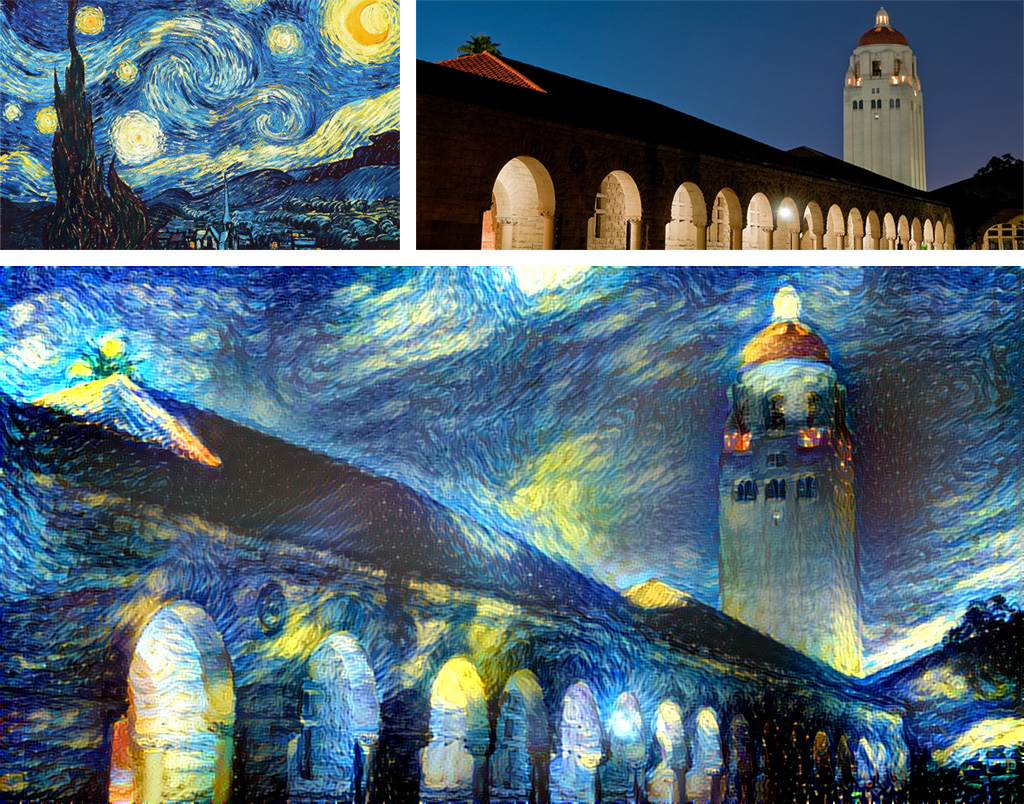
\includegraphics[width=\textwidth]{gfx/neural-style-composed}
  \caption{Gatys' algorithm implementation \cite{Johnson2015} results. \textbf{Top-left}: \textit{The Starry Night} by Vincent van Gogh, 1889, source of style. \textbf{Top-right}: night-time photograph of the Stanford campus, source of content. \textbf{Bottom}: Combination of style and content from images above.}
  \label{fig:sec:intro:neural-style}
\end{figure}

Gatys created a system that is able to compose the style and content of two arbitrary images into a new one, depicted in Figure~\ref{fig:sec:intro:neural-style}.
The system, instead of using a Deep Neural Network trained for that precise purpose, uses an already trained one on object recognition and as the network processes an image, its content and style are extracted separately from the intermediate layers.

This finding opens the door for wondering about other underlying understanding Deep Neural Networks develop as side effects, how this can be used to better understand the human brain \cite{Yamins2016}, or what other uses already trained networks may have.


% ------------------------------------------------------------------------------

\section{Goals}
\label{sec:intro:goals}

This supervised research project focuses on Gatys' unique approach for proving separation of form and content from the optic of Neural Networks. Being the field of Artificial Neural Networks extensive and in constant revision, in an effort to stay in topic the scope has been restricted to the following goals:

\begin{enumerate}
  \item Study the motivation and problematics of separation of form and content.
  \item Review how Machine Learning have approached separation of form and content.
  \item Understand how Deep Learning state of the art approaches separation of form and content.
  \item Find novel applications of state of the art approach.
  \item Propose improvements to the state of the art approach.
  \item Reflect on the implications of methods applied in state of the art approach.
\end{enumerate}


% ------------------------------------------------------------------------------

\section{Thesis Structure}
\label{sec:intro:structure}

\textbf{Chapter \ref{sec:theory}} \\[0.2em]
In chapter \ref{sec:theory} I briefly go over common concepts needed to understand the different approaches used for separation of style and content throughout history.

\textbf{Chapter \ref{sec:related}} \\[0.2em]
In chapter \ref{sec:related} I talk in more detail form and content, the motivation for having them separated, its problematics and how it has been traditionally approached by Machine Learning up to Gaty's work.

\textbf{Chapter \ref{sec:system}} \\[0.2em]
In chapter \ref{sec:system} I explain and discuss the results presented by \cite{Gatys2015}, as well as derived works.

\textbf{Chapter \ref{sec:conclusion}} \\[0.2em]
Finally, in chapter \ref{sec:conclusion} I will muse about the implications of Deep Neural Networks being able to extrapolate their past experience to tackle problems for which they weren't trained for.
